\documentclass[9pt,twoside,lineno]{pnas-new}
% Use the lineno option to display guide line numbers if required.

\templatetype{pnassupportinginfo}

% Math
\def\P{\mathbb{P}}
\def\cor{\mathrm{cor}}
\def\Quantile{\mathrm{Quantile}}
\def\logit{\mathrm{logit}}
\def\dist{\mathrm{dist}}
\def\WIS{\mathrm{WIS}}
\def\AUC{\mathrm{AUC}}
\newcommand{\indicator}[1]{\mathbf{1}\left(#1\right)}

% Figures and tables
\usepackage{xurl}
\usepackage{microtype}
\usepackage{booktabs}
\usepackage{caption}
\usepackage{subcaption}
\usepackage{xcolor}
\newcommand{\attn}[1]{\textcolor{red}{[ATTN: #1]}}

\makeatletter 
\renewcommand\@biblabel[1]{#1} 
\makeatother

% indicators
\newcommand{\chngcli}{CHNG-CLI}
\newcommand{\chngcov}{CHNG-COVID}
\newcommand{\dv}{DV-CLI}
\newcommand{\ar}{AR}
\newcommand{\fb}{CTIS-CLI-in-community}
\newcommand{\gs}{Google-AA}


\providecommand{\tightlist}{%
  \setlength{\itemsep}{0pt}\setlength{\parskip}{0pt}}


\title{Your main manuscript title}
\author{Author1, Author2 and Author3 (complete author list)}
\correspondingauthor{Corresponding Author name.\\E-mail: author.two@email.com}

\begin{document}



\instructionspage

\maketitle

\SItext

All our text goes here. Reference figures with the R chuck label as
Figure\textasciitilde{}\ref{fig:fcast-finalized}.

All figures go on their own page after all of the text\ldots{}

Edit \texttt{pnas-suppl-template.tex} for the correct Author list and
Title.

\hypertarget{examining-the-relative-advantage-of-using-finalized-rather-than-vintage-data}{%
\section{Examining the relative advantage of using finalized rather than
vintage
data}\label{examining-the-relative-advantage-of-using-finalized-rather-than-vintage-data}}

This section referes to
Figures\textasciitilde{}\ref{fig:fcast-finalized}--\ref{fig:hot-honest-v-finalized}.

\hypertarget{aggregating-with-geometric-mean}{%
\section{Aggregating with geometric
mean}\label{aggregating-with-geometric-mean}}

\begin{itemize}
\tightlist
\item
  The weighted interval score is bounded below by zero and can be very
  large. This behavior is typical of right-skewed distributions.
\item
  Figure\textasciitilde{}\ref{fig:wis-densities} illustrates that the
  densities appear log-Gaussian.
\item
  This suggests aggregating by the geometric mean rather than the mean
  for comparisons. See Figure\textasciitilde{}\ref{fig:fcast-adjusted}.
\end{itemize}

\hypertarget{bootstrap-results}{%
\section{Bootstrap results}\label{bootstrap-results}}

Here we discuss how implicit regularization is not the reason for
improved performance

\hypertarget{correlations-with-lagged-actuals}{%
\section{Correlations with lagged
actuals}\label{correlations-with-lagged-actuals}}

Alden's histograms are in Figure\textasciitilde{}\ref{fig:cor-wis-ratio}
and Figure\textasciitilde{}\ref{fig:cor-wis-ratio-m1}.

\hypertarget{upswings-and-downswings}{%
\section{Upswings and Downswings}\label{upswings-and-downswings}}

Logged version of Figure 5 in the manuscript is in
Figure\textasciitilde{}\ref{fig:upswing-histogram-logged}.

See also Table\textasciitilde{}\ref{tab:upswing-corr-table}.

\hypertarget{leadingness-and-laggingness}{%
\section{Leadingness and
laggingness}\label{leadingness-and-laggingness}}

Currently, both figures are in the manuscript. Probably just need text
here.

\hypertarget{examining-data-in-2021}{%
\section{Examining data in 2021}\label{examining-data-in-2021}}

See Figures \ref{fig:fcast-alldates} -- \ref{fig:hot-alldates}.

\hypertarget{deprecated}{%
\section{Deprecated}\label{deprecated}}

There are a few blocks at the bottom (figures with Google symptoms only
and the old trajectory plots) that we can remove once we decide.

\begin{figure}

{\centering 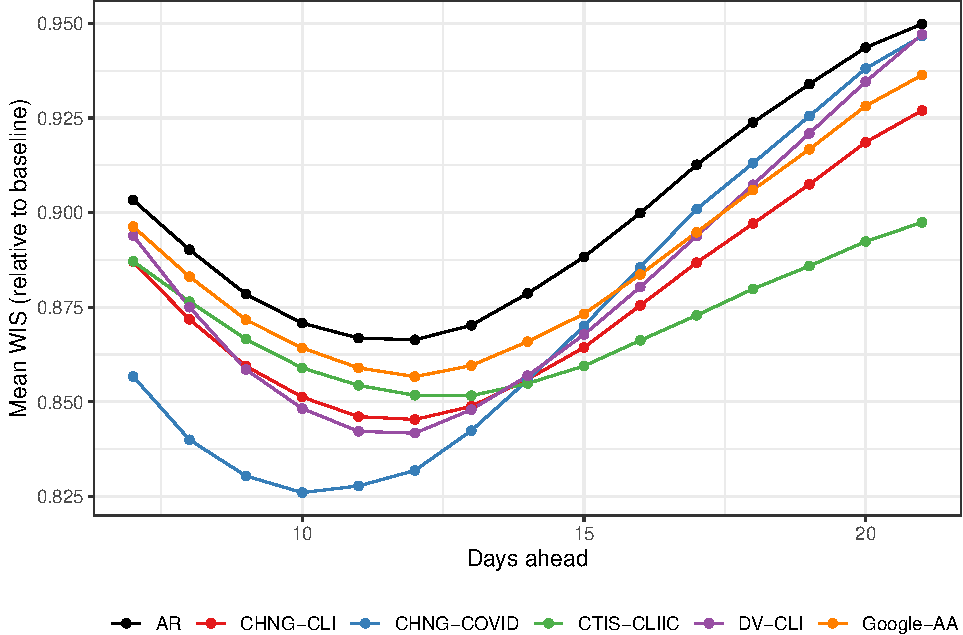
\includegraphics[width=\textwidth]{fig/fcast-finalized-1} 

}

\caption{Forecasting performance using finalized data. Compare to Figure 3 in the manuscript.}\label{fig:fcast-finalized}
\end{figure}

\clearpage

\begin{figure}

{\centering 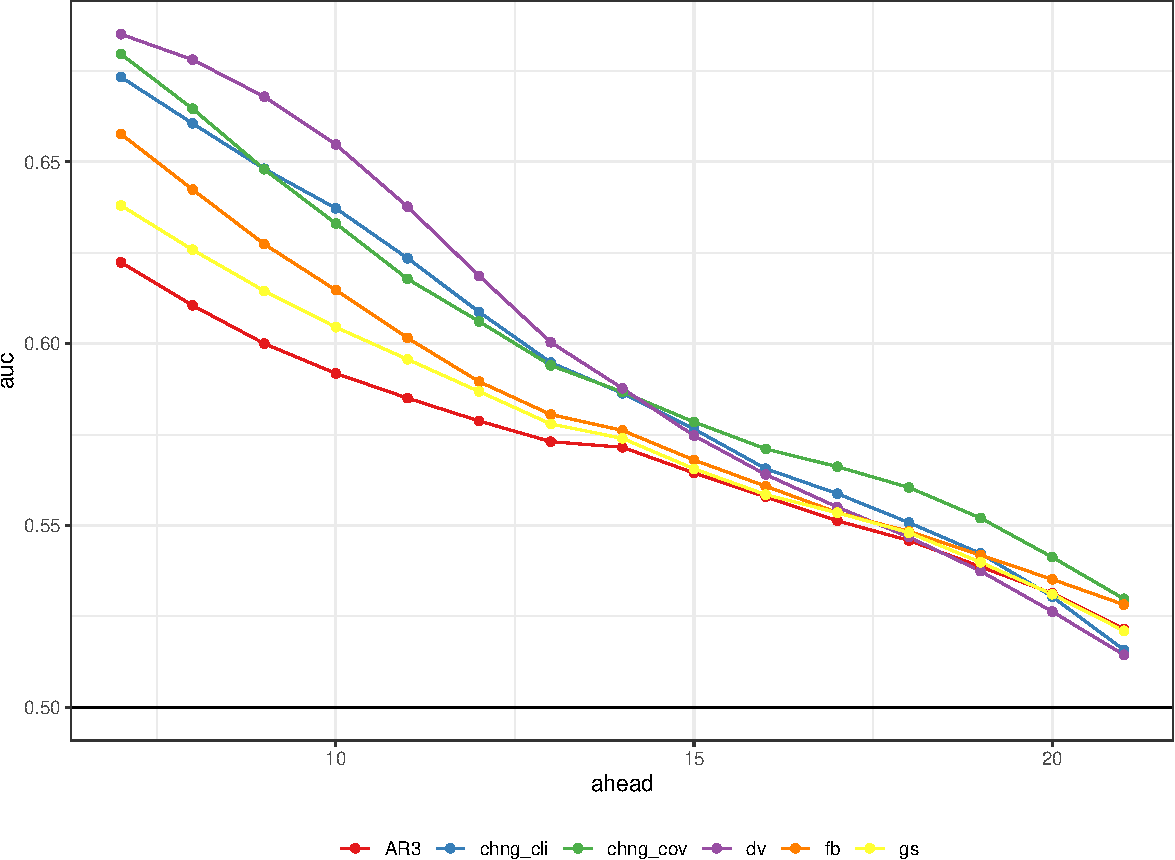
\includegraphics[width=\textwidth]{fig/hot-finalized-1} 

}

\caption{Hotspot prediction performance using finalized data. Compare to Figure 4 in the manuscript.}\label{fig:hot-finalized}
\end{figure}

\clearpage

\begin{figure}

{\centering 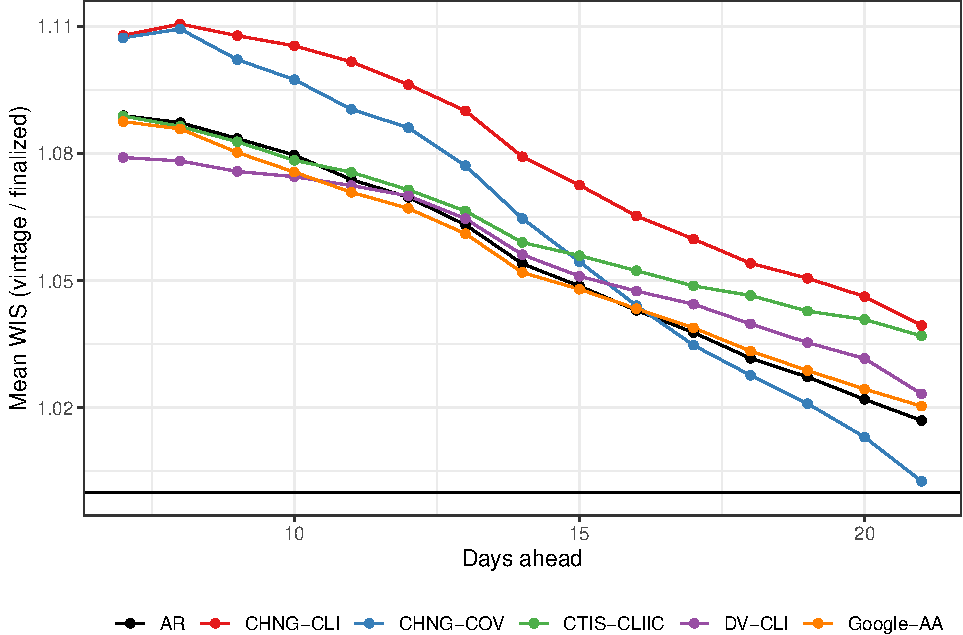
\includegraphics[width=\textwidth]{fig/fcast-honest-v-finalized-1} 

}

\caption{Relative forecast WIS with vintage compared to finalized data. Using finalized data leads to overly optimistic performance.}\label{fig:fcast-honest-v-finalized}
\end{figure}

\clearpage

\begin{figure}

{\centering 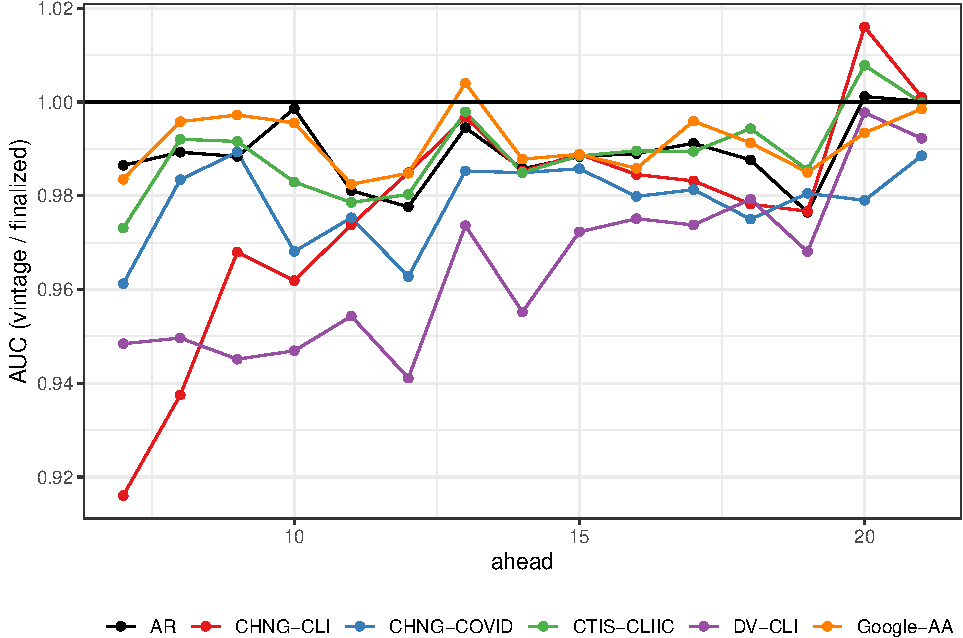
\includegraphics[width=\textwidth]{fig/hot-honest-v-finalized-1} 

}

\caption{Relative AUC with vintage compared to finalized data. Using finalized data leads to overly optimistic hotspot performance.}\label{fig:hot-honest-v-finalized}
\end{figure}

\clearpage

\begin{figure}

{\centering 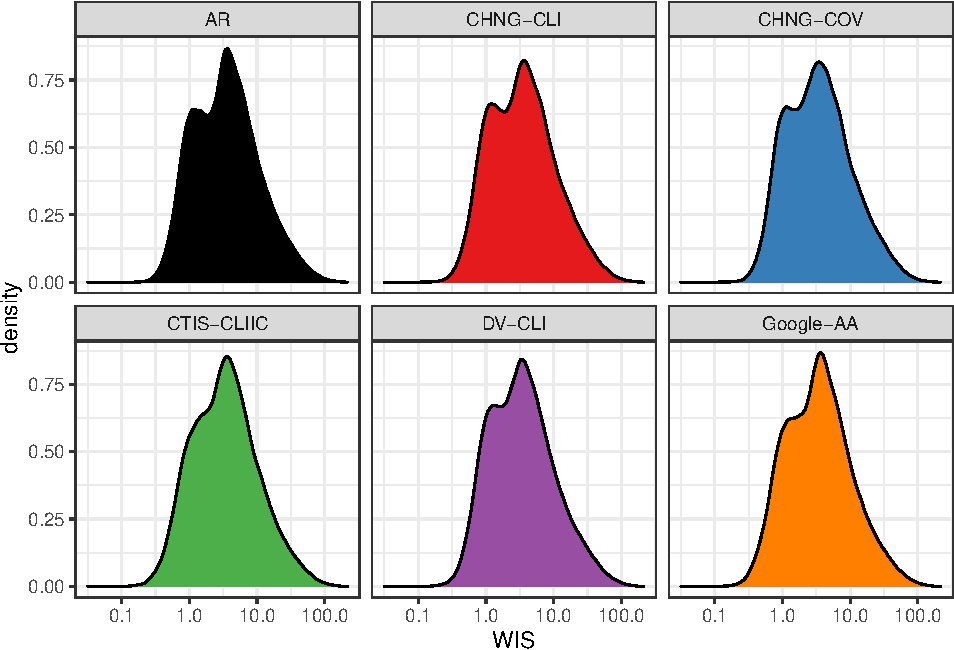
\includegraphics[width=\textwidth]{fig/wis-densities-1} 

}

\caption{Weighted interval score appears to more closely resemble a log-Gaussian distribution.}\label{fig:wis-densities}
\end{figure}

\clearpage

\begin{figure}

{\centering 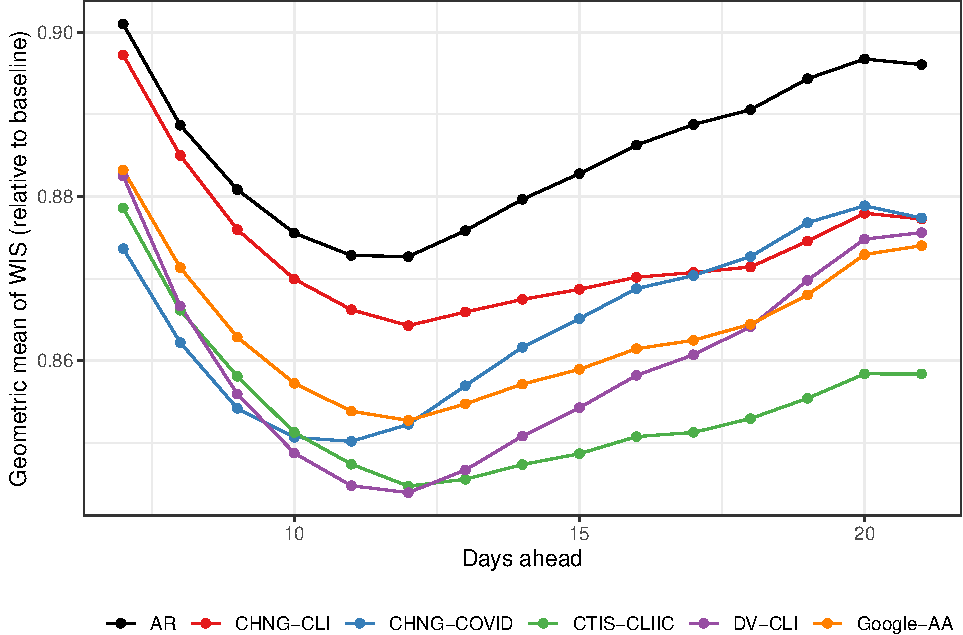
\includegraphics[width=\textwidth]{fig/fcast-adjusted-1} 

}

\caption{Relative forecast performance using vintage data and summarizing with the more robust geometric mean.}\label{fig:fcast-adjusted}
\end{figure}

\clearpage

\begin{figure}

{\centering 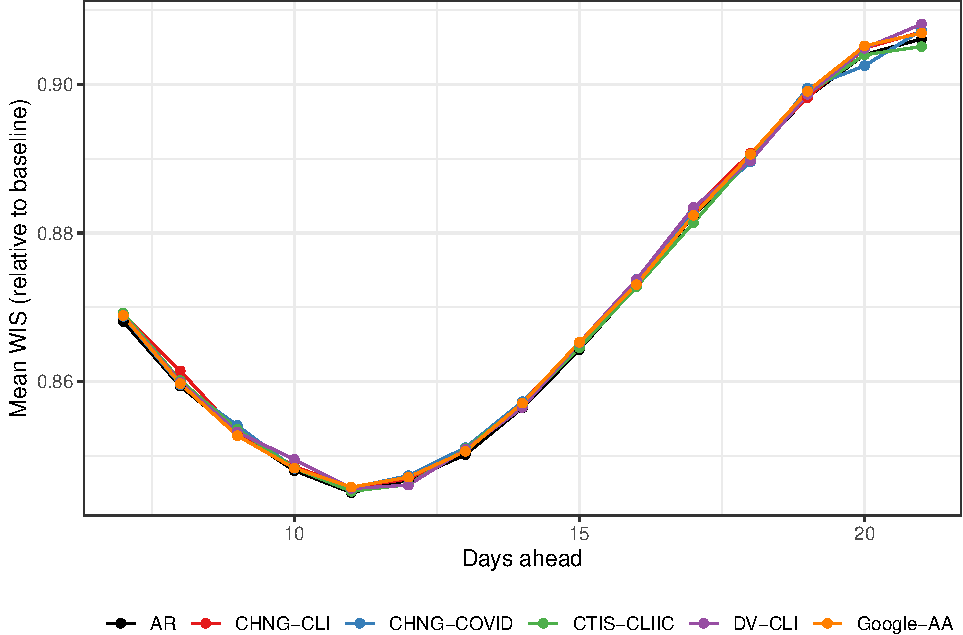
\includegraphics[width=\textwidth]{fig/fcast-booted-1} 

}

\caption{Forecast performance when indicators are replaced with samples from their empirical distribution. Performance is largely similar to the AR model.}\label{fig:fcast-booted}
\end{figure}

\clearpage

\begin{figure}

{\centering 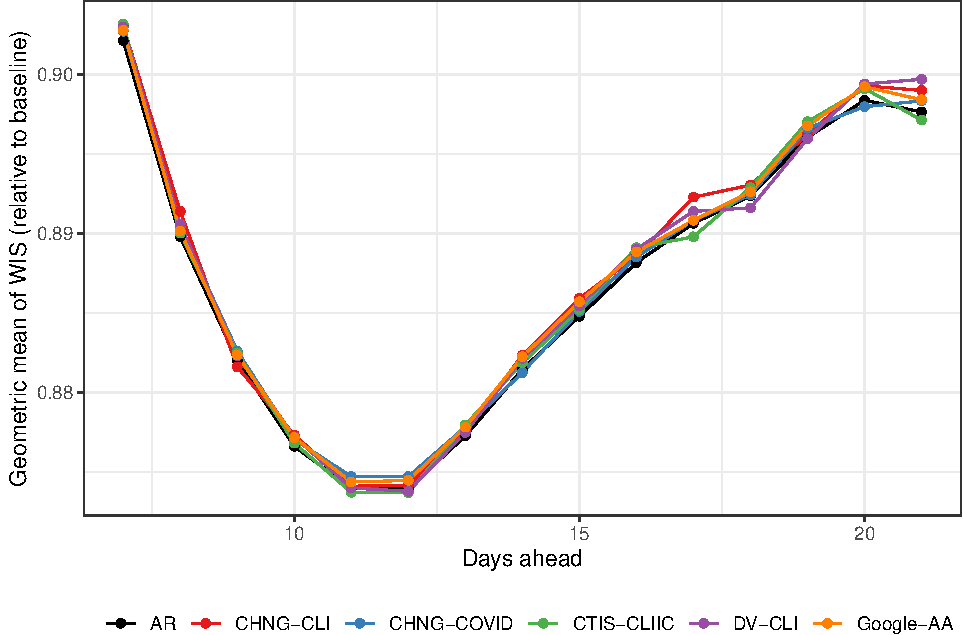
\includegraphics[width=\textwidth]{fig/fcast-booted-adjusted-1} 

}

\caption{Forecast performance as measured with the geometric mean when indicators are replaced with samples from their empirical distribution. Performance is largely similar to the AR model.}\label{fig:fcast-booted-adjusted}
\end{figure}

\clearpage

\begin{figure}

{\centering 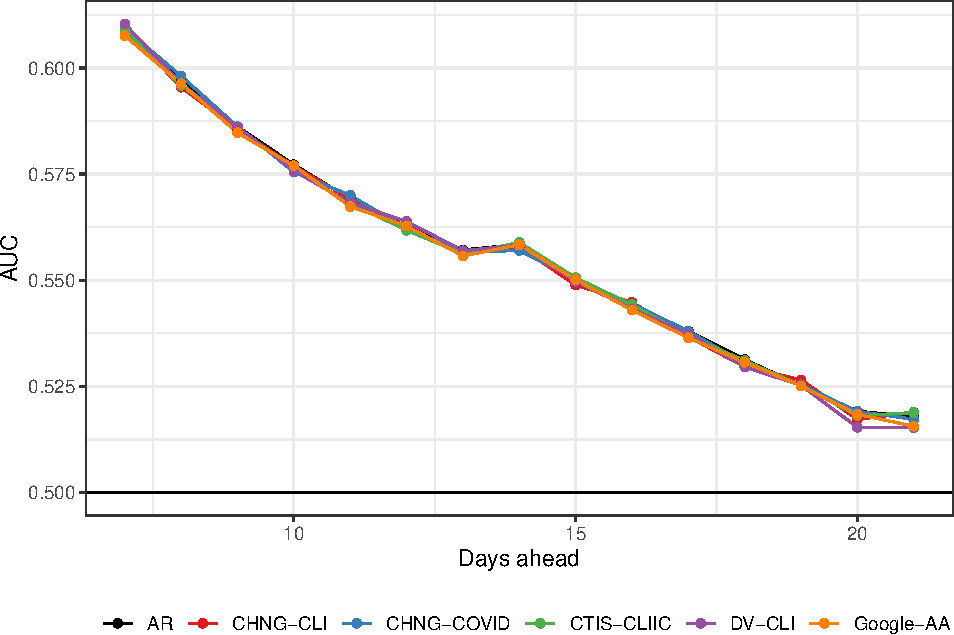
\includegraphics[width=\textwidth]{fig/hot-booted-1} 

}

\caption{Hotspot prediction performance when indicators are replaced with samples from their empirical distribution. Performance is largely similar to the AR model.}\label{fig:hot-booted}
\end{figure}

\clearpage

\begin{figure}

{\centering 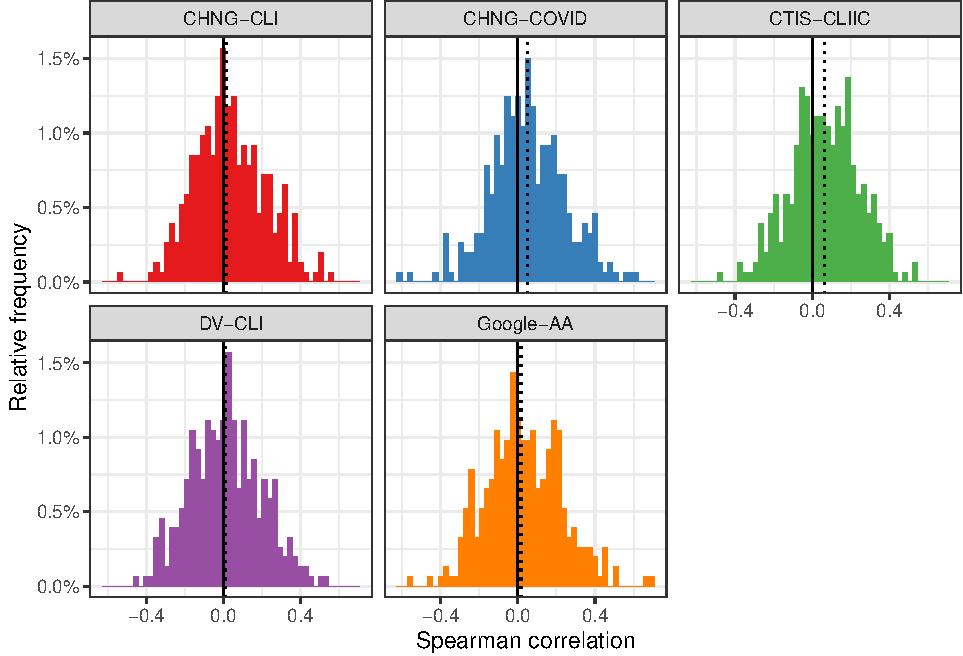
\includegraphics[width=\textwidth]{fig/cor-wis-ratio-1} 

}

\caption{This is one of the correlation plots Alden made. It shows histograms of the Spearman correlation between the ratio of AR to AR WIS with the percent change in 7dav cases relative to 7 days earlier.}\label{fig:cor-wis-ratio}
\end{figure}

\clearpage

\begin{figure}

{\centering 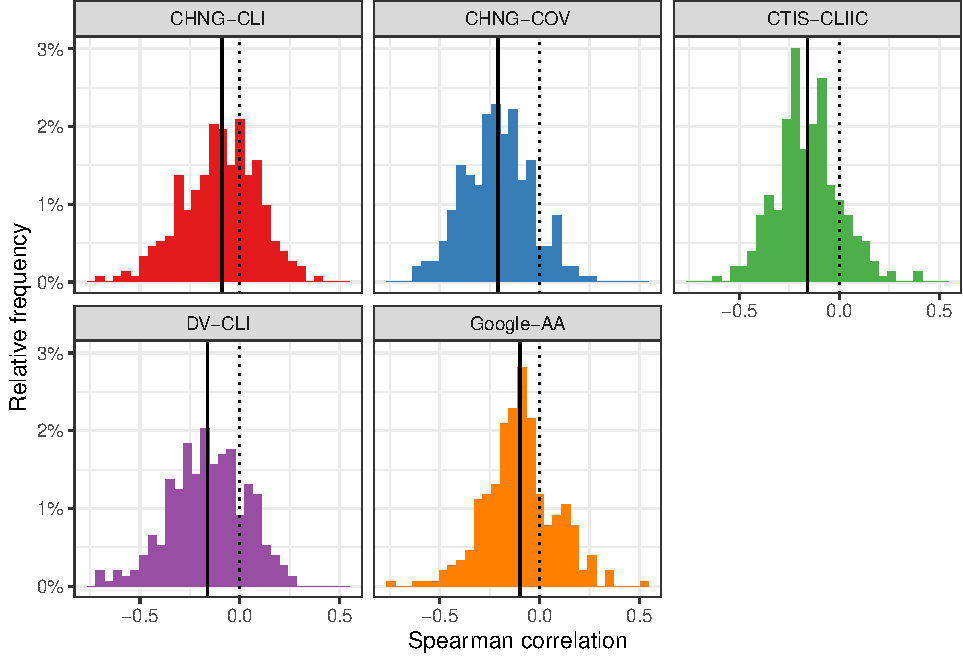
\includegraphics[width=\textwidth]{fig/cor-wis-ratio-m1-1} 

}

\caption{This is Alden's second set of histograms. Here we have the correlation of the absolute value of WIS ratio - 1 with the percent change in 7dav cases relative to 7 days earlier}\label{fig:cor-wis-ratio-m1}
\end{figure}

\clearpage

\begin{figure}

{\centering 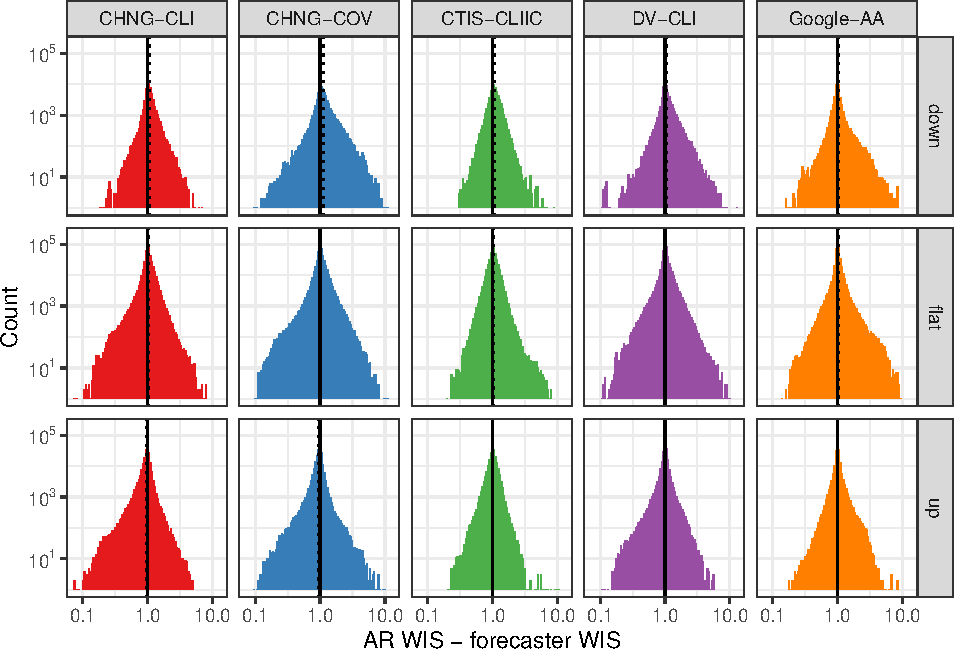
\includegraphics[width=\textwidth]{fig/upswing-histogram-logged-1} 

}

\caption{Not sure if we want this here. Similar to Figure 5 in the manuscript but taking logs. }\label{fig:upswing-histogram-logged}
\end{figure}

\clearpage

\begin{table}

\caption{\label{tab:upswing-corr-table}Correlation of the difference in WIS between the AR model with the difference in median predictions. In down periods, improvements in forecast risk are highly correlated with lower median predictions. The opposite is true in up periods. This suggests, as one might expect that improved performance of the indicator-assisted model is attributable to being closer to the truth then the AR model. This conclusion is stronger in down periods then in up periods.}
\centering
\begin{tabular}[t]{lrrrrr}
\toprule
udf & CHNG-CLI & CHNG-COVID & CTIS-CLIIC & DV-CLI & Google-AA\\
\midrule
down & 0.79 & 0.80 & 0.83 & 0.81 & 0.81\\
flat & 0.12 & 0.17 & 0.28 & 0.18 & 0.17\\
up & -0.57 & -0.56 & -0.53 & -0.53 & -0.47\\
\bottomrule
\end{tabular}
\end{table}

\clearpage

\begin{figure}

{\centering 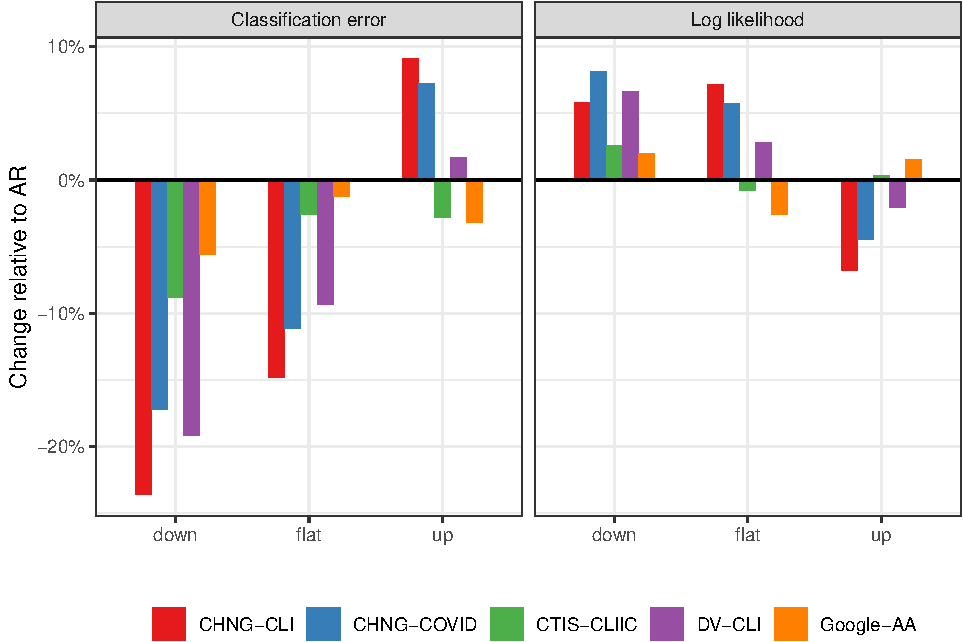
\includegraphics[width=\textwidth]{fig/hotspots-upswing-downswing-1} 

}

\caption{Classification and loglikelihood separated into periods of upswing, downswing, and flat cases. Like the analysis of the forecasting task in the main paper (see Figure 7), performance is better during down and flat periods.}\label{fig:hotspots-upswing-downswing}
\end{figure}

\clearpage

\begin{figure}

{\centering 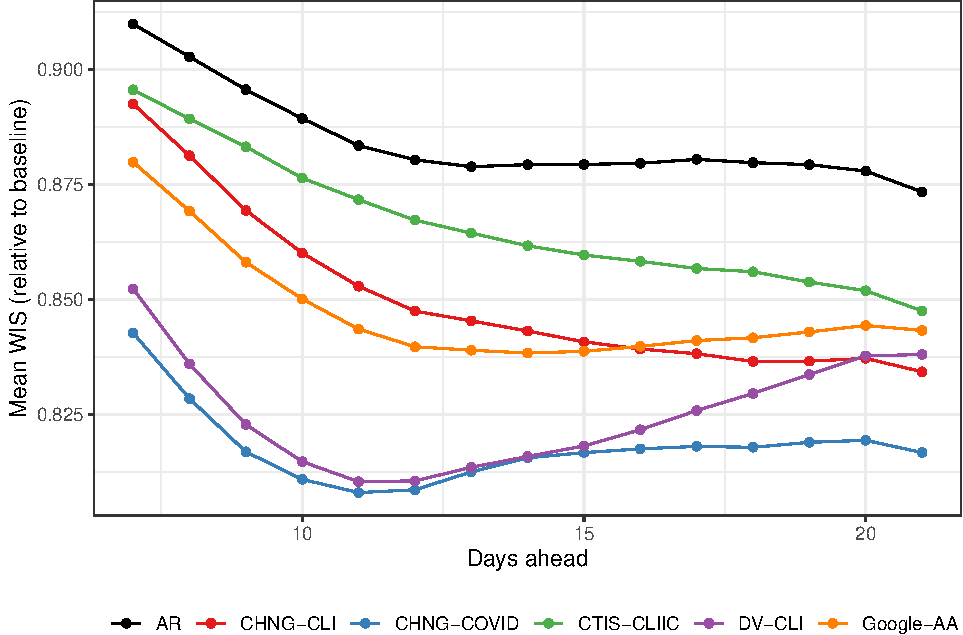
\includegraphics[width=\textwidth]{fig/fcast-alldates-1} 

}

\caption{Forecast performance over all periods. Performance largely improves for all forecasters with the inclusion of data in 2021.}\label{fig:fcast-alldates}
\end{figure}

\clearpage

\begin{figure}

{\centering 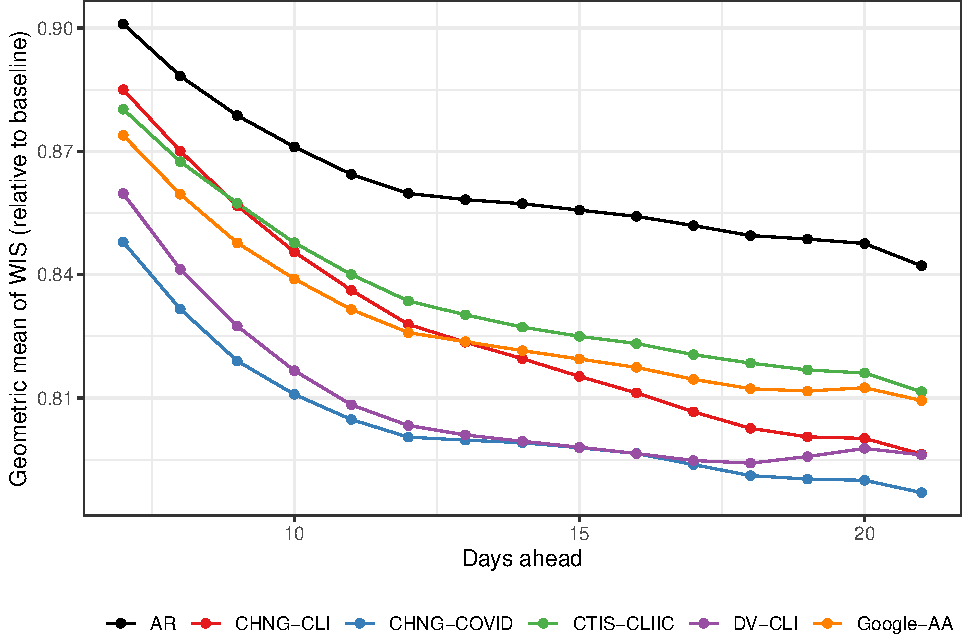
\includegraphics[width=\textwidth]{fig/fcast-alldates-adjusted-1} 

}

\caption{Forcast performance over all periods aggregaged with the geometric mean. Again, the inclusion of data in 2021 leads to improved performance.}\label{fig:fcast-alldates-adjusted}
\end{figure}

\clearpage

\begin{figure}

{\centering 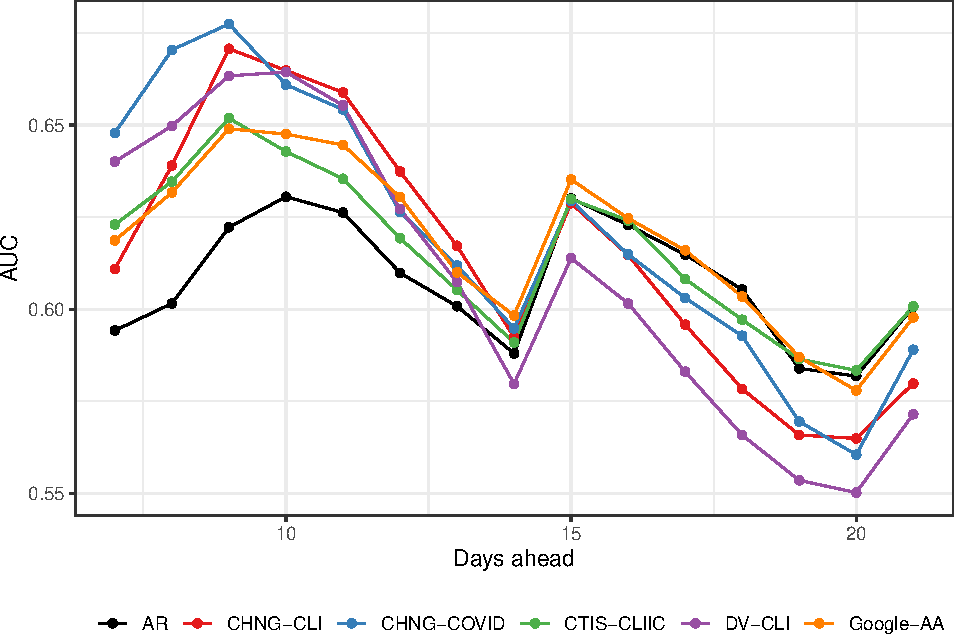
\includegraphics[width=\textwidth]{fig/hot-alldates-1} 

}

\caption{Area under the curve for hotspot predictions including data in 2021. Performance degrades relative to the period in 2020. However, there are far fewer hotspots during this period as case rates declined in much of the country.}\label{fig:hot-alldates}
\end{figure}

\clearpage

\clearpage

\FloatBarrier

\movie{Type legend for the movie here.}

\dataset{dataset_one.txt}{Type or paste legend here.}

\dataset{dataset_two.txt}{Type or paste legend here. Adding longer text to show what happens, to decide on alignment and/or indentations for multi-line or paragraph captions.}






\bibliography{../../common/covidcast.bib,pnas-materials/pnas-sample.bib}

\end{document}